\documentclass[9pt,aspectratio=169]{beamer}
\usetheme{Boadilla}
\usepackage[utf8]{inputenc}
\usepackage{amsmath,amssymb,amsfonts}
\usepackage{mathtools}
\usepackage{tikz}
\usetikzlibrary{arrows.meta,calc}

\title{Module 2: Linear Algebra}
\subtitle{Vectors, Transformations, Spaces \& Structures --- Exam Reference Notes}
\author{Mathematics for Computing}
% \date{\small Reference: Bronson, Costa \& Saccoman, \emph{Linear Algebra: Algorithms, Applications, and Techniques}, 4e, 2023}

\setbeamertemplate{footline}[frame number]
\setbeamertemplate{navigation symbols}{}

\newcommand{\keyidea}[1]{%
\par\medskip\noindent\textbf{Key Idea to Remember:} #1\par\medskip}

\newcommand{\childex}[1]{%
\par\medskip\noindent\textbf{In Plain Words:} #1\par\medskip}

\begin{document}

\begin{frame}
\titlepage
\end{frame}

\begin{frame}{Roadmap for Module 2}
\small
\begin{columns}[t]
\column{0.5\textwidth}
\begin{enumerate}
\item Algebraic Structures (Groups, Rings, Fields)
\item Vectors \& Coordinate Systems
\item Vector Addition
\item Scalar Multiplication
\item Linear Combinations, Span, Basis
\item Matrices as Transformations
\item 3D Linear Transformations
\item The Determinant
\item Inverse, Column Space, Null Space
\end{enumerate}
\column{0.5\textwidth}
\begin{enumerate}
\setcounter{enumi}{9}
\item Nonsquare Matrices Between Dimensions
\item Dot Product \& Duality
\item Hyperplanes
\item Cross Product
\item Cross Product via Transformations
\item Cramer's Rule
\item Change of Basis
\item Eigenvectors \& Eigenvalues
\item Vector Spaces
\item Mathematical Spaces
\end{enumerate}
\end{columns}
\end{frame}

% ================= SECTION 1: ALGEBRAIC STRUCTURES =================
\section{Algebraic Structures}

\begin{frame}{Algebraic Structures}


\par\noindent\textbf{Definition: Algebraic Structure.}\par
An algebraic structure is a pair $(S, *)$ where $S$ is a non-empty set and
$* : S \times S \to S$ is a binary operation on $S$ (i.e., combining two elements of $S$
always gives another element of $S$ --- this is called \emph{closure}).
\medskip

\keyidea{Every "number system" you use in linear algebra (integers, reals, vectors,
matrices) is an algebraic structure whose behaviour is fixed by a short list of axioms.
Learn the axioms once, and you understand every structure built on top of them.}
\end{frame}

\begin{frame}{Groups}
\par\noindent\textbf{Definition: Group.}\par
A set $G$ with operation $*$ is a \textbf{group} $(G,*)$ if:
\begin{enumerate}
\item \textbf{Closure:} $a*b \in G$ for all $a,b \in G$
\item \textbf{Associativity:} $(a*b)*c = a*(b*c)$
\item \textbf{Identity:} $\exists\, e \in G$ such that $a*e = e*a = a$
\item \textbf{Inverse:} $\forall a \in G,\ \exists\, a^{-1} \in G$ such that $a*a^{-1}=e$
\end{enumerate}
If also $a*b = b*a$ for all $a,b$, the group is \textbf{abelian} (commutative).
\medskip


\par\noindent\textbf{Example.}\par
$(\mathbb{R}, +)$ is an abelian group: identity is $0$, inverse of $a$ is $-a$.
$(\mathbb{R}^n, +)$ --- ordinary vector addition --- is also an abelian group: this is
exactly why "vectors can be added and undone" always works.
\medskip


\childex{Think of a group like a locked room with a return ticket: whatever move you make
($*$), you can always find a move that brings you back to where you started (inverse), and
there is always a "do nothing" move (identity).}
\end{frame}

\begin{frame}{Rings and Fields}
\par\noindent\textbf{Definition: Ring.}\par
A \textbf{ring} $(R, +, \cdot)$ is a set with two operations such that $(R,+)$ is an
abelian group, $\cdot$ is associative, and $\cdot$ distributes over $+$:
$a\cdot(b+c) = a\cdot b + a\cdot c$.
\medskip


\par\noindent\textbf{Definition: Field.}\par
A \textbf{field} $(F,+,\cdot)$ is a ring in which $(F\setminus\{0\}, \cdot)$ is also an
abelian group (every non-zero element has a multiplicative inverse). Example: $\mathbb{R}$,
$\mathbb{C}$, $\mathbb{Q}$.
\medskip


\keyidea{A \textbf{vector space} (Slide 18) is always defined "over a field" --- the
scalars you are allowed to multiply vectors by must come from a field, because you need to
add, subtract, multiply, and divide those scalars safely. This is the direct link between
Section 1 and everything that follows.}
\end{frame}

% ================= SECTION 2: VECTORS =================
\section{Vectors and Coordinate Systems}

\begin{frame}{Vectors and Coordinate Systems}
\footnotesize
\begin{columns}[T]
\begin{column}{0.56\textwidth}
\par\noindent\textbf{Definition.}\par
A \textbf{vector} in $\mathbb{R}^n$ is an ordered $n$-tuple of real numbers, written as a
column: $\mathbf{v} = (v_1, v_2, \dots, v_n)$. Geometrically it is an arrow starting at the
origin of a \textbf{coordinate system} and ending at the point $(v_1,\dots,v_n)$.
\medskip

\childex{Imagine standing at a crossroads (the origin). A vector is an instruction:
"walk 3 steps East, then 4 steps North."}

\par\noindent\textbf{Example.}\par
$\mathbf{v} = (3,4)$: move 3 units along $x$, 4 units along $y$.
Length $\|\mathbf{v}\| = \sqrt{3^2+4^2} = 5$.
\medskip

\keyidea{A vector has both \textbf{magnitude} (length) and \textbf{direction} --- it is an
arrow from the origin to a point, not just the point itself.}
\end{column}
\begin{column}{0.42\textwidth}
\centering
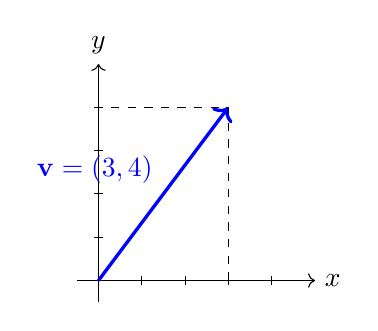
\begin{tikzpicture}[scale=0.55]
\draw[->] (-0.5,0) -- (5,0) node[right]{$x$};
\draw[->] (0,-0.5) -- (0,5) node[above]{$y$};
\foreach \x in {1,2,3,4} \draw (\x,0.1)--(\x,-0.1);
\foreach \y in {1,2,3,4} \draw (0.1,\y)--(-0.1,\y);
\draw[->,very thick,blue] (0,0) -- (3,4) node[midway,above left]{$\mathbf{v}=(3,4)$};
\draw[dashed] (3,0)--(3,4)--(0,4);
\end{tikzpicture}
\\[0.3em]{\scriptsize $\mathbf{v}$ as an arrow on the coordinate grid}
\end{column}
\end{columns}
\end{frame}

% ================= SECTION 3: VECTOR ADDITION =================
\section{Vector Addition}

\begin{frame}{Vector Addition}
\footnotesize
\begin{columns}[T]
\begin{column}{0.56\textwidth}
\par\noindent\textbf{Definition.}\par
For $\mathbf{u}=(u_1,\dots,u_n)$ and $\mathbf{v}=(v_1,\dots,v_n)$:
\[ \mathbf{u} + \mathbf{v} = (u_1+v_1,\ u_2+v_2,\ \dots,\ u_n+v_n) \]
Geometrically: place the tail of $\mathbf{v}$ at the head of $\mathbf{u}$; the sum is the
arrow from the start of $\mathbf{u}$ to the end of $\mathbf{v}$ (\emph{tip-to-tail rule}).
\medskip

\par\noindent\textbf{Example.}\par
$\mathbf{u}=(1,2),\ \mathbf{v}=(3,-1) \Rightarrow \mathbf{u}+\mathbf{v}=(4,1)$.
\medskip

\childex{Doing "walk 1 East, 2 North" then "walk 3 East, 1 South" is the same as one
combined instruction: "walk 4 East, 1 North."}

\keyidea{Vector addition is just adding matching coordinates --- the operation that makes
$(\mathbb{R}^n, +)$ a group (Slide 3).}
\end{column}
\begin{column}{0.42\textwidth}
\centering
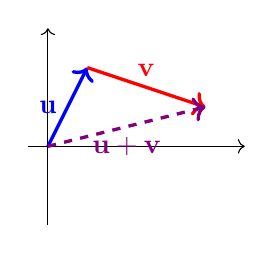
\begin{tikzpicture}[scale=0.5]
\draw[->] (-0.5,0) -- (5,0);
\draw[->] (0,-2) -- (0,3);
\draw[->,very thick,blue] (0,0) -- (1,2) node[midway,left]{$\mathbf{u}$};
\draw[->,very thick,red] (1,2) -- (4,1) node[midway,above]{$\mathbf{v}$};
\draw[->,very thick,violet,dashed] (0,0) -- (4,1) node[midway,below]{$\mathbf{u}+\mathbf{v}$};
\end{tikzpicture}
\\[0.3em]{\scriptsize Tip-to-tail addition}
\end{column}
\end{columns}
\end{frame}

% ================= SECTION 4: SCALAR MULTIPLICATION =================
\section{Vector (Scalar) Multiplication}

\begin{frame}{Scalar Multiplication}
\footnotesize
\begin{columns}[T]
\begin{column}{0.56\textwidth}
\par\noindent\textbf{Definition.}\par
For a scalar $c \in \mathbb{R}$ and vector $\mathbf{v}=(v_1,\dots,v_n)$:
\[ c\mathbf{v} = (cv_1, cv_2, \dots, cv_n) \]
It scales the length of $\mathbf{v}$ by $|c|$; if $c<0$, the direction reverses.
\medskip

\par\noindent\textbf{Example.}\par
$\mathbf{v}=(2,3)$, $c=3 \Rightarrow 3\mathbf{v}=(6,9)$ (same direction, 3$\times$ longer).
$c=-1 \Rightarrow -\mathbf{v}=(-2,-3)$ (opposite direction, same length).
\medskip

\childex{Scalar multiplication is a zoom slider: turn it up and the arrow stretches; make
it negative and the arrow flips backward.}

\keyidea{Addition + scalar multiplication together are called \textbf{linear operations}
--- nearly every idea in this module builds from just these two moves.}
\end{column}
\begin{column}{0.42\textwidth}
\centering
\begin{tikzpicture}[scale=0.42]
\draw[->] (-3,0) -- (7,0);
\draw[->] (0,-4) -- (0,10);
\draw[->,very thick,blue] (0,0) -- (2,3) node[right]{$\mathbf{v}$};
\draw[->,very thick,red] (0,0) -- (6,9) node[right]{$3\mathbf{v}$};
\draw[->,very thick,violet] (0,0) -- (-2,-3) node[left]{$-\mathbf{v}$};
\end{tikzpicture}
\\[0.3em]{\scriptsize Scaling stretches; a negative sign flips direction}
\end{column}
\end{columns}
\end{frame}

% ================= SECTION 5: LINEAR COMBINATIONS, SPAN, BASIS =================
\section{Linear Combinations, Span and Basis}

\begin{frame}{Linear Combinations and Span}
\footnotesize
\begin{columns}[T]
\begin{column}{0.56\textwidth}
\par\noindent\textbf{Definition.}\par
A \textbf{linear combination} of vectors $\mathbf{v}_1,\dots,\mathbf{v}_k$ is
$c_1\mathbf{v}_1 + c_2\mathbf{v}_2 + \dots + c_k\mathbf{v}_k$ for scalars $c_i$.
The \textbf{span} of $\{\mathbf{v}_1,\dots,\mathbf{v}_k\}$ is the set of \emph{all}
possible linear combinations of them.
\medskip

\par\noindent\textbf{Example.}\par
$\text{span}\{(1,0),(0,1)\} = \mathbb{R}^2$ (every point reachable).
$\text{span}\{(1,2)\}$ is just the line through the origin with slope $2$.
\medskip

\childex{With only "walk East" and "walk North" (any amount, even negative), the span is
every location reachable using just those two tools.}

\keyidea{Span answers: \emph{"What is the largest region I can reach using only these
vectors?"}}
\end{column}
\begin{column}{0.42\textwidth}
\centering
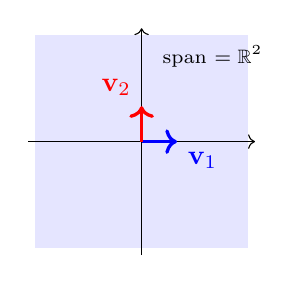
\begin{tikzpicture}[scale=0.45]
\fill[blue!10] (-3,-3) rectangle (3,3);
\draw[->] (-3.2,0) -- (3.2,0);
\draw[->] (0,-3.2) -- (0,3.2);
\draw[->,very thick,blue] (0,0) -- (1,0) node[below right]{$\mathbf{v}_1$};
\draw[->,very thick,red] (0,0) -- (0,1) node[above left]{$\mathbf{v}_2$};
\node at (2,2.4) {\scriptsize span $=\mathbb{R}^2$};
\end{tikzpicture}
\\[0.3em]{\scriptsize Two independent vectors span the whole plane}
\end{column}
\end{columns}
\end{frame}

\begin{frame}{Basis Vectors}
\par\noindent\textbf{Definition.}\par
A set $\{\mathbf{b}_1,\dots,\mathbf{b}_n\}$ is a \textbf{basis} of a space $V$ if:
\begin{enumerate}
\item it \textbf{spans} $V$ (reaches everywhere in $V$), and
\item it is \textbf{linearly independent} (no vector in the set is a combination of the
others --- none is "wasted").
\end{enumerate}
\medskip


\par\noindent\textbf{Example.}\par
$\{(1,0),(0,1)\}$ is the \textbf{standard basis} of $\mathbb{R}^2$: minimal, spans
everything. $\{(1,0),(0,1),(1,1)\}$ spans $\mathbb{R}^2$ too, but is \textbf{not} a basis
--- it has one vector too many (not independent).
\medskip


\keyidea{A basis is the \textbf{smallest possible toolkit} of vectors that can still build
every vector in the space. The number of vectors in a basis is the \textbf{dimension} of
the space.}
\end{frame}

% ================= SECTION 6: MATRICES AS TRANSFORMATIONS =================
\section{Matrices as Linear Transformations}

\begin{frame}{Matrices as Linear Transformations}
\footnotesize
\begin{columns}[T]
\begin{column}{0.56\textwidth}
\par\noindent\textbf{Definition.}\par
A matrix $A$ is a rectangular array of numbers. Multiplying $A\mathbf{x}$ takes a vector
$\mathbf{x}$ and moves it to a new vector --- this is called a \textbf{linear
transformation}. The columns of $A$ tell you exactly where the basis vectors land.
\medskip

\par\noindent\textbf{Example.}\par
$A = \begin{pmatrix} 2 & 0 \\ 0 & 3 \end{pmatrix}$ sends $(1,0)\mapsto(2,0)$ and
$(0,1)\mapsto(0,3)$: stretches the plane 2$\times$ horizontally, 3$\times$ vertically.
\medskip

\childex{A matrix is a recipe card: "wherever the basis arrows used to point, here is
where they point now."}

\keyidea{$A\mathbf{x}$ is a \textbf{picture-moving machine} that keeps grid lines
straight, evenly spaced, and passing through the origin.}
\end{column}
\begin{column}{0.42\textwidth}
\centering
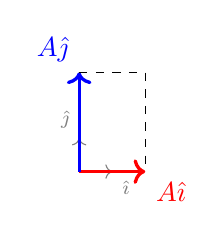
\begin{tikzpicture}[scale=0.42]
\draw[->,gray] (0,0) -- (1,0) node[below right]{\scriptsize$\hat\imath$};
\draw[->,gray] (0,0) -- (0,1) node[above left]{\scriptsize$\hat\jmath$};
\draw[->,very thick,red] (0,0) -- (2,0) node[below right]{$A\hat\imath$};
\draw[->,very thick,blue] (0,0) -- (0,3) node[above left]{$A\hat\jmath$};
\draw[dashed] (0,3)--(2,3)--(2,0);
\end{tikzpicture}
\\[0.3em]{\scriptsize Basis vectors land at the matrix's columns}
\end{column}
\end{columns}
\end{frame}

\begin{frame}{Matrix Multiplication as Composition}
\par\noindent\textbf{Definition.}\par
If $A$ and $B$ are matrices, the product $AB$ represents applying transformation $B$
\textbf{first}, then $A$: $(AB)\mathbf{x} = A(B\mathbf{x})$.
\medskip


\par\noindent\textbf{Example.}\par
Let $B$ rotate the plane $90^\circ$, and $A$ stretch it 2$\times$. Then $AB\mathbf{x}$
means: first rotate, then stretch. In general $AB \neq BA$ --- order matters!
\medskip


\childex{Think of two instructions on a robot arm: "rotate, then stretch" usually gives a
different final pose than "stretch, then rotate." Matrix multiplication records exactly
this order.}

\keyidea{Matrix multiplication = doing one transformation right after another. This is why
matrix multiplication is \textbf{associative} $(AB)C=A(BC)$ but generally \textbf{not
commutative} $AB \neq BA$.}
\end{frame}

% ================= SECTION 7: 3D TRANSFORMATIONS =================
\section{Three-Dimensional Linear Transformations}

\begin{frame}{Three-Dimensional Linear Transformations}
\small
\par\noindent\textbf{Definition.}\par
A linear transformation $T:\mathbb{R}^3 \to \mathbb{R}^3$ is represented by a $3\times 3$
matrix. Each column shows where $\hat{\imath}=(1,0,0)$, $\hat{\jmath}=(0,1,0)$,
$\hat{k}=(0,0,1)$ land after the transformation.
\medskip


\par\noindent\textbf{Example.}\par
\[
A = \begin{pmatrix} 1&0&0\\0&1&0\\0&0&2\end{pmatrix}
\]
stretches only the $z$-direction by 2$\times$, leaving the $xy$-plane untouched --- like
squashing or stretching a block of clay along one axis.
\medskip


\childex{Everything that worked for a flat 2D grid (Slide 8) works the same way in 3D ---
you just now have three basis directions to track instead of two, so the "recipe card"
matrix has three columns.}

\keyidea{Extending from 2D to 3D changes \emph{how much} bookkeeping you do, but not the
\emph{idea}: a matrix always tells you where the basis vectors go.}
\end{frame}

% ================= SECTION 8: DETERMINANT =================
\section{The Determinant}

\begin{frame}{The Determinant}
\footnotesize
\begin{columns}[T]
\begin{column}{0.56\textwidth}
\par\noindent\textbf{Definition (2$\times$2).}\par
For $A = \begin{pmatrix} a&b\\c&d\end{pmatrix}$, $\det(A) = ad-bc$.
Measures the \textbf{scaling factor of area} (2D) or \textbf{volume} (3D) caused by $A$.
\medskip

\par\noindent\textbf{Example.}\par
$A = \begin{pmatrix} 2&0\\0&3\end{pmatrix} \Rightarrow \det(A) = 6$: a unit square becomes
a rectangle with 6$\times$ the area. If $\det(A)=0$, space is squashed into a lower
dimension --- all area/volume destroyed.
\medskip

\childex{Photocopying a picture 2$\times$ wider and 3$\times$ taller covers $6\times$ the
paper. The determinant is exactly this "area multiplier," negative if the map also flips
(mirrors) space.}

\keyidea{$\det(A)=0 \iff$ columns of $A$ are dependent $\iff$ $A$ is \textbf{not
invertible}.}
\end{column}
\begin{column}{0.42\textwidth}
\centering
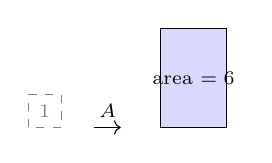
\begin{tikzpicture}[scale=0.42]
\draw[gray,dashed] (0,0) rectangle (1,1);
\node[gray] at (0.5,0.5) {\scriptsize 1};
\draw[->] (2,0) -- (2.8,0) node[midway,above]{\scriptsize$A$};
\fill[blue!15] (4,0) rectangle (6,3);
\draw (4,0) rectangle (6,3);
\node at (5,1.5) {\scriptsize area $=6$};
\end{tikzpicture}
\\[0.3em]{\scriptsize Unit square $\to$ area scaled by $\det(A)$}
\end{column}
\end{columns}
\end{frame}

% ================= SECTION 9: INVERSE, COLUMN SPACE, NULL SPACE =================
\section{Inverse Matrices, Column Space and Null Space}

\begin{frame}{Inverse Matrices}
\par\noindent\textbf{Definition.}\par
The \textbf{inverse} $A^{-1}$ of a square matrix $A$ satisfies $AA^{-1}=A^{-1}A=I$ (the
identity matrix). It exists \textbf{iff} $\det(A)\neq 0$. Solving $A\mathbf{x}=\mathbf{b}$
becomes $\mathbf{x}=A^{-1}\mathbf{b}$.
\medskip


\par\noindent\textbf{Example.}\par
$A=\begin{pmatrix}2&0\\0&3\end{pmatrix} \Rightarrow A^{-1}=\begin{pmatrix}1/2&0\\0&1/3
\end{pmatrix}$ --- it exactly \textbf{undoes} the stretching done by $A$.
\medskip


\childex{If $A$ is a transformation that "stretches 2$\times$ sideways, 3$\times$ up",
then $A^{-1}$ is the "un-stretch" that shrinks everything back to exactly where it
started.}
\end{frame}

\begin{frame}{Column Space and Null Space}
\par\noindent\textbf{Definition.}\par
\textbf{Column space} $\text{Col}(A)$: the span of $A$'s columns --- i.e., every possible
output $A\mathbf{x}$ can land in.
\textbf{Null space} $\text{Null}(A)$: all $\mathbf{x}$ such that $A\mathbf{x}=\mathbf{0}$
--- the vectors that get squashed to the origin.
\medskip


\par\noindent\textbf{Example.}\par
$A=\begin{pmatrix}1&2\\2&4\end{pmatrix}$: both columns point the same direction, so
$\text{Col}(A)$ is just a line, not the whole plane. Its null space is the line
$x_1 = -2x_2$ --- every point on that line is crushed to $(0,0)$.
\medskip


\keyidea{\textbf{Rank--Nullity Theorem:} $\dim(\text{Col}(A)) + \dim(\text{Null}(A)) = n$
(number of columns). Column space measures "where you can land"; null space measures
"what gets lost."}
\end{frame}

% ================= SECTION 10: NONSQUARE MATRICES =================
\section{Nonsquare Matrices Between Dimensions}

\begin{frame}{Nonsquare Matrices as Transformations Between Dimensions}
\par\noindent\textbf{Definition.}\par
An $m \times n$ matrix ($m \neq n$) represents a transformation
$T:\mathbb{R}^n \to \mathbb{R}^m$ --- it changes the number of dimensions, not just the
shape of the space.
\medskip


\par\noindent\textbf{Example.}\par
$A = \begin{pmatrix} 1 & 0 \\ 0 & 1 \\ 1 & 1 \end{pmatrix}$ is $3\times 2$: it takes a 2D
input and produces a 3D output --- it "lifts" a flat plane into 3D space (input dimension
$2 <$ output dimension $3$).
A $2\times 3$ matrix instead \textbf{flattens} 3D space onto a 2D plane, like a shadow.
\medskip


\keyidea{A matrix does not need to be square! Rows = dimension of the output space,
columns = dimension of the input space. Rectangular matrices move information
\textbf{between} different-sized spaces.}
\end{frame}

% ================= SECTION 11: DOT PRODUCT AND DUALITY =================
\section{Dot Product and Duality}

\begin{frame}{Dot Product}
\begin{columns}[T]
\begin{column}{0.56\textwidth}
\par\noindent\textbf{Definition.}\par
$\mathbf{u}\cdot\mathbf{v} = u_1v_1 + u_2v_2 + \dots + u_nv_n =
\|\mathbf{u}\|\,\|\mathbf{v}\|\cos\theta$, where $\theta$ is the angle between them.
\medskip

\par\noindent\textbf{Example.}\par
$\mathbf{u}=(1,2),\ \mathbf{v}=(3,-1) \Rightarrow \mathbf{u}\cdot\mathbf{v}=1(3)+2(-1)=1$.
If $\mathbf{u}\cdot\mathbf{v}=0$, the vectors are \textbf{perpendicular}.
\medskip

\childex{The dot product answers: "how much does one arrow point in the same direction as
another?" Big positive = same way; zero = right angles; negative = somewhat opposite.}
\end{column}
\begin{column}{0.42\textwidth}
\centering
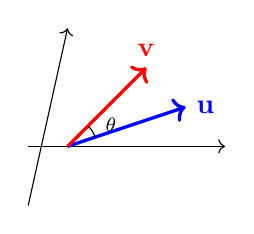
\begin{tikzpicture}[scale=0.5]
\draw[->] (-1,0) -- (4,0);
\draw[->] (-1,-1.5) -- (0,3);
\draw[->,very thick,blue] (0,0) -- (3,1) node[right]{$\mathbf{u}$};
\draw[->,very thick,red] (0,0) -- (2,2) node[above]{$\mathbf{v}$};
\draw (0.7,0.23) arc (18:45:0.7);
\node at (1.1,0.55) {\scriptsize$\theta$};
\end{tikzpicture}
\\[0.3em]{\scriptsize Angle $\theta$ between $\mathbf{u}$ and $\mathbf{v}$}
\end{column}
\end{columns}
\end{frame}

\begin{frame}{Duality}
\par\noindent\textbf{Definition.}\par
Every linear transformation $\mathbb{R}^n \to \mathbb{R}$ (a "linear functional") can be
written as a dot product with some fixed vector $\mathbf{u}$: $T(\mathbf{v}) =
\mathbf{u}\cdot\mathbf{v}$. This $\mathbf{u}$ is the \textbf{dual vector} of $T$.
\medskip


\par\noindent\textbf{Example.}\par
The $1\times 2$ matrix $(2\ \ 3)$ acting on $(x,y)$ gives $2x+3y$ --- identical to
$(2,3)\cdot(x,y)$. The "row matrix" and the "vector" are secretly the same object viewed
two ways.
\medskip


\keyidea{\textbf{Duality} is the surprising fact that "linear transformations that output
a single number" and "vectors" are two sides of the same coin --- every such
transformation \emph{is} a dot product with a specific vector.}
\end{frame}

% ================= SECTION 12: HYPERPLANES (NEW) =================
\section{Hyperplanes}

\begin{frame}{Hyperplanes}
\footnotesize
\begin{columns}[T]
\begin{column}{0.56\textwidth}
\par\noindent\textbf{Definition.}\par
A \textbf{hyperplane} in $\mathbb{R}^n$ is a flat subset of dimension $n-1$: the solution
set of one linear equation
$\mathbf{n}\cdot\mathbf{x} = c$, $\mathbf{n}\neq \mathbf{0}$,
where $\mathbf{n}$ is the \textbf{normal vector} (perpendicular to it) and $c$ a constant.
\medskip

\par\noindent\textbf{Example.}\par
In $\mathbb{R}^2$, a hyperplane is a \textbf{line}: $2x+3y=6$ has normal $\mathbf{n}=(2,3)$.
In $\mathbb{R}^3$, it is an ordinary \textbf{plane}: $x+y+z=1$.
\medskip

\childex{A point cuts a line, a line cuts a plane, a plane cuts 3D space --- the normal
vector is a flagpole sticking straight out, showing which way is "up" from it.}

\keyidea{A hyperplane through the origin is exactly the \textbf{null space} (Slide 9) of
$\mathbf{x}\mapsto \mathbf{n}\cdot\mathbf{x}$ --- also the key object behind decision
boundaries in ML classifiers.}
\end{column}
\begin{column}{0.42\textwidth}
\centering
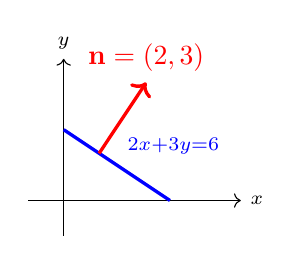
\begin{tikzpicture}[scale=0.45]
\draw[->] (-1,0) -- (5,0) node[right]{\scriptsize$x$};
\draw[->] (0,-1) -- (0,4) node[above]{\scriptsize$y$};
\draw[very thick,blue] (0,2) -- (3,0) node[midway,above right]{\scriptsize$2x{+}3y{=}6$};
\draw[->,very thick,red] (1,1.33) -- (2.33,3.33) node[above]{$\mathbf{n}=(2,3)$};
\end{tikzpicture}
\\[0.3em]{\scriptsize Line = hyperplane in $\mathbb{R}^2$; $\mathbf{n}$ perpendicular to it}
\end{column}
\end{columns}
\end{frame}

% ================= SECTION 13: CROSS PRODUCT =================
\section{Cross Product}

\begin{frame}{Cross Product}
\footnotesize
\begin{columns}[T]
\begin{column}{0.56\textwidth}
\par\noindent\textbf{Definition.}\par
For $\mathbf{u},\mathbf{v}\in\mathbb{R}^3$:
\[
\mathbf{u}\times\mathbf{v} =
\left(u_2v_3-u_3v_2,\ u_3v_1-u_1v_3,\ u_1v_2-u_2v_1\right)
\]
A new vector \textbf{perpendicular to both} $\mathbf{u}$ and $\mathbf{v}$, with length
$\|\mathbf{u}\|\|\mathbf{v}\|\sin\theta$ = area of the parallelogram they span.
\medskip

\par\noindent\textbf{Example.}\par
$\mathbf{u}=(1,0,0),\ \mathbf{v}=(0,1,0) \Rightarrow \mathbf{u}\times\mathbf{v}=(0,0,1)$
--- perpendicular to the $xy$-plane, pointing "up," by the right-hand rule.
\medskip

\childex{Only in 3D does "perpendicular to two arrows" pin a unique direction. Point your
right-hand fingers from $\mathbf{u}$ to $\mathbf{v}$; your thumb shows
$\mathbf{u}\times\mathbf{v}$.}
\end{column}
\begin{column}{0.42\textwidth}
\centering
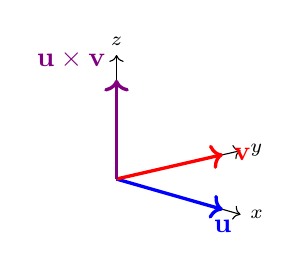
\begin{tikzpicture}[scale=0.45]
\draw[->] (0,0) -- (3.5,-1) node[right]{\scriptsize$x$};
\draw[->] (0,0) -- (3.5,0.8) node[right]{\scriptsize$y$};
\draw[->] (0,0) -- (0,3.5) node[above]{\scriptsize$z$};
\draw[->,very thick,blue] (0,0) -- (3,-0.86) node[below]{$\mathbf{u}$};
\draw[->,very thick,red] (0,0) -- (3,0.69) node[right]{$\mathbf{v}$};
\draw[->,very thick,violet] (0,0) -- (0,2.8) node[above left]{$\mathbf{u}\times\mathbf{v}$};
\end{tikzpicture}
\\[0.3em]{\scriptsize Right-hand rule: perpendicular to $\mathbf{u}$ and $\mathbf{v}$}
\end{column}
\end{columns}
\end{frame}

% ================= SECTION 14: CROSS PRODUCT VIA TRANSFORMATIONS =================
\section{Cross Product via Linear Transformations}

\begin{frame}{Cross Products in the Light of Linear Transformations}
\par\noindent\textbf{Definition.}\par
$\mathbf{u}\times\mathbf{v}$ can be defined via a determinant / dual-vector trick:
define the linear functional $T(\mathbf{x}) = \det[\mathbf{x}\ \ \mathbf{u}\ \
\mathbf{v}]$ (a $3\times3$ determinant with $\mathbf{x}$ as first column). By duality
(Slide 11), $T(\mathbf{x}) = \mathbf{p}\cdot\mathbf{x}$ for a unique $\mathbf{p}$ --- and
that $\mathbf{p}$ is exactly $\mathbf{u}\times\mathbf{v}$.
\medskip


\keyidea{This reframes the cross product as: \emph{"the vector whose dot product with
anything equals the signed volume of the parallelepiped formed with $\mathbf{u}$ and
$\mathbf{v}$."} It elegantly ties together determinants (Slide 8), duality (Slide 11), and
the cross product into one idea.}

\childex{Instead of memorising the messy cross-product formula, remember: it is "the
special vector that reports volumes" --- built from the determinant, discovered using the
duality trick.}
\end{frame}

% ================= SECTION 15: CRAMER'S RULE =================
\section{Cramer's Rule}

\begin{frame}{Cramer's Rule}
\small
\par\noindent\textbf{Definition.}\par
For $A\mathbf{x}=\mathbf{b}$ with $\det(A)\neq 0$, each unknown is:
\[ x_i = \frac{\det(A_i)}{\det(A)} \]
where $A_i$ is $A$ with column $i$ replaced by $\mathbf{b}$.
\medskip


\par\noindent\textbf{Example.}\par
$\begin{cases}2x+y=5\\x-y=1\end{cases}$, $A=\begin{pmatrix}2&1\\1&-1\end{pmatrix}$,
$\det(A)=-3$. Replacing column 1 with $(5,1)$: $\det(A_1) = -6 \Rightarrow x = 2$.
Replacing column 2: $\det(A_2) = -3 \Rightarrow y = 1$.
\medskip


\childex{Cramer's Rule uses the determinant's "area/volume" meaning (Slide 8): swapping in
$\mathbf{b}$ and comparing the new volume to the old volume directly tells you each
unknown's value --- no elimination steps needed.}

\keyidea{Cramer's Rule is elegant for small systems and for theory, but computationally
expensive for large $n$; Gaussian elimination is faster in practice.}
\end{frame}

% ================= SECTION 16: CHANGE OF BASIS =================
\section{Change of Basis}

\begin{frame}{Change of Basis}
\par\noindent\textbf{Definition.}\par
If $B=\{\mathbf{b}_1,\dots,\mathbf{b}_n\}$ is a basis, any vector $\mathbf{v}$ can be
written in \textbf{$B$-coordinates}. The \textbf{change-of-basis matrix} $P$ (whose
columns are the $\mathbf{b}_i$, written in the standard basis) converts between the two:
\[ \mathbf{v}_{\text{standard}} = P\,\mathbf{v}_{B}, \qquad
\mathbf{v}_{B} = P^{-1}\mathbf{v}_{\text{standard}} \]
\medskip


\par\noindent\textbf{Example.}\par
New basis $\mathbf{b}_1=(2,1),\ \mathbf{b}_2=(-1,1)$. A vector that is "$(1,1)$ in the new
basis" corresponds to $1\cdot\mathbf{b}_1 + 1\cdot\mathbf{b}_2 = (1,2)$ in the standard
coordinates.
\medskip


\childex{Changing basis is like converting temperature between Celsius and Fahrenheit ---
same physical reality (the same arrow), described using a different scale/grid.}

\keyidea{To translate a transformation matrix $A$ (given in the standard basis) into the
new basis $B$, use $A_B = P^{-1}AP$.}
\end{frame}

% ================= SECTION 17: EIGENVECTORS AND EIGENVALUES =================
\section{Eigenvectors and Eigenvalues}

\begin{frame}{Eigenvectors and Eigenvalues}
\footnotesize
\begin{columns}[T]
\begin{column}{0.56\textwidth}
\par\noindent\textbf{Definition.}\par
For a square matrix $A$, a nonzero vector $\mathbf{v}$ is an \textbf{eigenvector} with
\textbf{eigenvalue} $\lambda$ if:
\[ A\mathbf{v} = \lambda \mathbf{v} \]
$A$ only \textbf{stretches/shrinks} $\mathbf{v}$ (by factor $\lambda$) --- it does
\textbf{not} rotate it off its own line. Found by solving $\det(A-\lambda I)=0$
(the \textbf{characteristic equation}).
\medskip

\par\noindent\textbf{Example.}\par
$A=\begin{pmatrix}2&0\\0&3\end{pmatrix}$: eigenvectors $(1,0)$ with $\lambda=2$, and
$(0,1)$ with $\lambda=3$ --- the axes don't rotate, only stretch.
\medskip

\childex{Most vectors get knocked off their line by a transformation. Eigenvectors are the
rare directions that stay on the \textbf{same line}, just longer or shorter --- like the
axis a spinning top wobbles around.}
\end{column}
\begin{column}{0.42\textwidth}
\centering
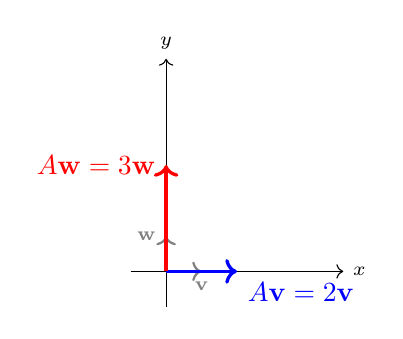
\begin{tikzpicture}[scale=0.45]
\draw[->] (-1,0) -- (5,0) node[right]{\scriptsize$x$};
\draw[->] (0,-1) -- (0,6) node[above]{\scriptsize$y$};
\draw[->,thick,gray] (0,0) -- (1,0) node[below]{\scriptsize$\mathbf{v}$};
\draw[->,very thick,blue] (0,0) -- (2,0) node[below right]{$A\mathbf{v}=2\mathbf{v}$};
\draw[->,thick,gray] (0,0) -- (0,1) node[left]{\scriptsize$\mathbf{w}$};
\draw[->,very thick,red] (0,0) -- (0,3) node[left]{$A\mathbf{w}=3\mathbf{w}$};
\end{tikzpicture}
\\[0.3em]{\scriptsize Eigenvectors stay on their own line, only scaled}
\end{column}
\end{columns}
\end{frame}

\begin{frame}{Diagonalization}
\keyidea{If a matrix $A$ has enough independent eigenvectors, we can write
$A = PDP^{-1}$, where $D$ is diagonal (eigenvalues on the diagonal) and $P$'s columns are
the eigenvectors. This is exactly a \textbf{change of basis} (Slide 16) into "eigenvector
coordinates," where the messy transformation $A$ becomes simple scaling $D$.}

\par\noindent\textbf{Why it matters.}\par
Diagonalization makes repeated transformations trivial: $A^k = PD^kP^{-1}$, and $D^k$ is
just each diagonal entry raised to the power $k$ --- used constantly in algorithms
(e.g., PCA, Markov chains, PageRank).
\medskip

\end{frame}

% ================= SECTION 18: VECTOR SPACES =================
\section{Vector Spaces}

\begin{frame}{Vector Spaces --- Axioms}
\par\noindent\textbf{Definition.}\par
A \textbf{vector space} $V$ over a field $F$ (Slide 4) is a set with addition and scalar
multiplication satisfying 8 axioms, including:
\begin{itemize}
\item $(V,+)$ is an abelian group (closure, associativity, identity $\mathbf{0}$, inverses)
\item $1\cdot\mathbf{v}=\mathbf{v}$; $\ (ab)\mathbf{v}=a(b\mathbf{v})$
\item Distributivity: $a(\mathbf{u}+\mathbf{v})=a\mathbf{u}+a\mathbf{v}$,\
$(a+b)\mathbf{v}=a\mathbf{v}+b\mathbf{v}$
\end{itemize}
\medskip


\par\noindent\textbf{Example.}\par
$\mathbb{R}^n$ is the classic vector space. Less obvious examples: the set of all
polynomials of degree $\le 2$, or the set of all $2\times2$ matrices --- both satisfy every
axiom, so both are legitimate "vector spaces," even though their elements are not arrows.
\medskip


\keyidea{Once a system obeys these 8 rules, \textbf{everything} we built in this
module --- span, basis, linear transformations, eigenvectors --- automatically applies to
it, whether the "vectors" are arrows, polynomials, or matrices.}
\end{frame}

\begin{frame}{Subspaces}
\par\noindent\textbf{Definition.}\par
A \textbf{subspace} $W\subseteq V$ is a subset that is itself a vector space: it must
contain $\mathbf{0}$, and be closed under addition and scalar multiplication.
\medskip


\par\noindent\textbf{Example.}\par
Any line or plane through the origin in $\mathbb{R}^3$ is a subspace. The column space and
null space (Slide 9) are both subspaces --- one of the output space, one of the input
space.
\medskip


\childex{A subspace is a "space within a space" that never lets you leave through addition
or scaling --- it must include the origin, since $0\cdot\mathbf{v}=\mathbf{0}$ always.}
\end{frame}

% ================= SECTION 19: MATHEMATICAL SPACES (NEW) =================
\section{Mathematical Spaces}

\begin{frame}{Mathematical Spaces: The Bigger Picture}
\childex{A vector space (Slide 18) tells you how to add and scale. But it says nothing
about "distance" or "angle" between two elements. \textbf{Mathematical spaces} add extra
structure on top of a set to capture ideas like closeness, length, and angle.}

\par\noindent\textbf{Definition: Metric Space.}\par
A \textbf{metric space} $(X,d)$ is a set $X$ with a distance function $d:X\times X \to
\mathbb{R}_{\ge0}$ satisfying: $d(x,y)=0 \iff x=y$; symmetry $d(x,y)=d(y,x)$; and the
triangle inequality $d(x,z)\le d(x,y)+d(y,z)$.
\medskip


\par\noindent\textbf{Example.}\par
$\mathbb{R}^n$ with $d(\mathbf{x},\mathbf{y})=\|\mathbf{x}-\mathbf{y}\|$ (ordinary
distance) is a metric space. So is a city grid using "taxicab distance"
$|x_1-y_1|+|x_2-y_2|$ --- a different, but still valid, notion of distance.
\medskip

\end{frame}

\begin{frame}{Normed and Inner Product Spaces}
\par\noindent\textbf{Definition: Normed Space.}\par
A \textbf{norm} $\|\cdot\|$ assigns a non-negative "length" to each vector, satisfying
$\|\mathbf{v}\|=0\iff \mathbf{v}=\mathbf{0}$, $\|c\mathbf{v}\|=|c|\|\mathbf{v}\|$, and the
triangle inequality. A vector space with a norm is a \textbf{normed space}; every norm
automatically gives a metric via $d(\mathbf{u},\mathbf{v})=\|\mathbf{u}-\mathbf{v}\|$.
\medskip


\par\noindent\textbf{Definition: Inner Product Space.}\par
An \textbf{inner product} $\langle \cdot,\cdot\rangle$ generalises the dot product
(Slide 11) to any vector space, satisfying linearity, symmetry, and positive-definiteness.
It gives both a norm ($\|\mathbf{v}\|=\sqrt{\langle\mathbf{v},\mathbf{v}\rangle}$) and a
notion of \textbf{angle}.
\medskip


\keyidea{The chain of generality is: \textbf{Inner Product Space} $\Rightarrow$
\textbf{Normed Space} $\Rightarrow$ \textbf{Metric Space}. Each step keeps less structure:
angle and length $\to$ only length $\to$ only distance. $\mathbb{R}^n$ with the dot product
sits at the richest end of this chain --- which is exactly why it is the space used
throughout this module.}
\end{frame}

% ================= SUMMARY =================
\begin{frame}{Module 2: Summary}
\small
\begin{itemize}
\item \textbf{Algebraic structures} (group/ring/field) give the rules of arithmetic that
vectors and scalars must obey.
\item \textbf{Vectors} live in a \textbf{coordinate system}; \textbf{addition} and
\textbf{scalar multiplication} are the two basic legal moves.
\item \textbf{Span} and \textbf{basis} describe what region vectors can reach, and the
minimal toolkit to reach it.
\item \textbf{Matrices} are transformations; \textbf{multiplication} is composing them;
this extends unchanged from 2D to 3D and to \textbf{nonsquare} maps between dimensions.
\item \textbf{Determinant} measures area/volume scaling and invertibility; \textbf{inverse},
\textbf{column space}, and \textbf{null space} describe what a matrix can undo, reach, and
destroy.
\item \textbf{Dot product} and \textbf{duality} connect vectors to linear functionals;
\textbf{hyperplanes} are the level sets of those functionals.
\item \textbf{Cross product} builds a perpendicular vector using exactly this duality
trick with determinants.
\item \textbf{Cramer's Rule} solves systems directly via determinants; \textbf{change of
basis} re-expresses everything in a new coordinate grid.
\item \textbf{Eigenvectors/eigenvalues} find the directions a transformation merely
scales; \textbf{vector spaces} and \textbf{mathematical spaces} generalise all of the above
beyond arrows in $\mathbb{R}^n$.
\end{itemize}
\end{frame}

\begin{frame}{Reference}
% \par\noindent\textbf{Primary Text.}\par
% Bronson, R., Costa, G.B., Saccoman, J.T. and Gross, D. \emph{Linear Algebra: Algorithms,
% Applications, and Techniques}, 4th Edition, 2023.
% \medskip

% \vspace{1em}
\centering
\Large End of Module 2 Notes
\end{frame}

\end{document}